% Chapter Template

\chapter{t-SNE} % Main chapter title

\label{Chapter8} % Change X to a consecutive number; for referencing this chapter elsewhere, use \ref{ChapterX}

%----------------------------------------------------------------------------------------
%	SECTION 1
%----------------------------------------------------------------------------------------

\section{Introduction}

The load profiles can present data in a new, previously unseen way, that can enable users or algorithms to extract patterns.
One such example would be when checking how similar are certain usage patterns.
This could be usage patterns within a household, where we are grouping appliances that are used similarly,
or when multiple buildings and how their consumption differs. 

Although the use-cases were presented in-depth in a separate chapter, it is worth mentioning one specific use case and this is energy poverty detection. 
The increasing price of energy resources, could lead to over-saving and living in cool homes.
Using similarity metrics between profiles across different buildings, it would be possible to detect outliers when it comes to heating the room. 
Using this technique it would be possible to detect users, that are living in below-average cool homes, and offer them cheaper plans. 

To measure the similarity of activation profiles, the t-SNE algorithm will be implemented.

\section{Goals}

The chapter will demonstrate the usefulness of previously unused load profiles, and show the practical use case using a t-SNE neighboring algorithm.

\section*{Methodology}

\subsection{Load profiles}

Based on the table of proposed profiles, the following profiles will be used in testing.
During testing, one of the proposed profiles will be used.
This is a weekly-daily load profile constructed from a month of data. 
Since there are roughly 4 weeks in each month, each pixel will present 4 samples. 

\subsubsection{Per-building}
This load profile is useful when it comes to comparing how activation patterns change over buildings and datasets.
insert example here
\subsubsection{Per-building Per-appliance}
This load profile is useful when comparing how usage is similar across buildings, and when
comparing a single appliance across many buildings. 
insert example here

\subsubsection{Bag-of-appliances}
This load profile is a combination of the load profiles above,
except it offers a larger detail when observing groups of appliances.
Since we are using one dimension for appliances, we will use only the daily dimension.
insert example here

\subsection{Datasets}
This section will be described in larger detail in the following chapter.

\subsection{t-SNE}

t-SNE or t-distribution stochastic neighboring embedding.

\section{Results}

\subsection{Results for per-building}
test
\begin{figure}[H]
	\centering
	\caption{"Per building data for all buildings"}
	\includegraphics[width=1.2\textwidth]{Figures/TSNE/TSNE_per_building/non_norm/scatter_non_norm_all.png}
	\label{fig:tsne_scatter_non_norm_all}
\end{figure}

\begin{figure}[H]
	\centering
	\caption{"Per building data for all buildings images"}
	\includegraphics[width=.9\textwidth]{Figures/TSNE/TSNE_per_building/non_norm/img_scatter_allall.png}
	\label{fig:tsne_pb_img_scatter_allall}
\end{figure}

\subsubsection{Normalise samples}

To make the image clearer I've normalized results and used only REFIT data, that
way it will be easier to read from legend. By normalising the algorithn
finds other ways to seperate the data.

\begin{figure}[H]
	\centering
	\caption{"Per building data for all buildings"}
	\includegraphics[width=1.2\textwidth]{Figures/TSNE/TSNE_per_building/all/scatter_all_all.png}
	\label{fig:tsne_pb_scatter_all_all}
\end{figure}

\begin{figure}[H]
	\centering
	\caption{"Per building data for refit buildings images"}
	\includegraphics[width=.9\textwidth]{Figures/TSNE/TSNE_per_building/all/img_scatter_allall.png}
	\label{fig:tsne_pb_img_scatter_allall}
\end{figure}


\section{Per-appliance}

\subsection{fridge}
Fridges are generally the same 

\begin{figure}[H]
	\centering
	\caption{"Per appliance data for all buildings"}
	\includegraphics[width=1.2\textwidth]{Figures/TSNE/TSNE_per_appliance/all/scatter_all_fridge_freeezer_fridge freezer.png}
	\label{fig:tsne_pa_scatter_all_fridge}
\end{figure}

\begin{figure}[H]
	\centering
	\caption{"Per appliance data for refit buildings images"}
	\includegraphics[width=.9\textwidth]{Figures/TSNE/TSNE_per_appliance/all/img_scatter_allfridge_freeezer_fridge freezer.png}
	\label{fig:tsne_pa_img_scatter_all_fridge}
\end{figure}


\subsection{kettle}
kettles are differnet

\begin{figure}[H]
	\centering
	\caption{"Per appliance data for all buildings"}
	\includegraphics[width=1.2\textwidth]{Figures/TSNE/TSNE_per_appliance/all/scatter_all_kettle.png}
	\label{fig:tsne_pa_scatter_all_kettle}
\end{figure}

\begin{figure}[H]
	\centering
	\caption{"Per appliance data for refit buildings images"}
	\includegraphics[width=.9\textwidth]{Figures/TSNE/TSNE_per_appliance/all/img_scatter_allkettle.png}
	\label{fig:tsne_pa_img_scatter_all_kettle}
\end{figure}

\subsection{microwave}
microwaves are differnet

\begin{figure}[H]
	\centering
	\caption{"Per appliance data for all buildings"}
	\includegraphics[width=1.2\textwidth]{Figures/TSNE/TSNE_per_appliance/all/scatter_all_microwave.png}
	\label{fig:tsne_pa_scatter_all_microwave}
\end{figure}

\begin{figure}[H]
	\centering
	\caption{"Per appliance data for refit buildings images"}
	\includegraphics[width=.9\textwidth]{Figures/TSNE/TSNE_per_appliance/all/img_scatter_allmicrowave.png}
	\label{fig:tsne_pa_img_scatter_all_microwave}
\end{figure}

\subsection{television}
tvs are different

\begin{figure}[H]
	\centering
	\caption{"Per appliance data for all buildings"}
	\includegraphics[width=1.2\textwidth]{Figures/TSNE/TSNE_per_appliance/all/scatter_all_television.png}
	\label{fig:tsne_pa_scatter_all_tv}
\end{figure}

\begin{figure}[H]
	\centering
	\caption{"Per appliance data for refit buildings images"}
	\includegraphics[width=.9\textwidth]{Figures/TSNE/TSNE_per_appliance/all/img_scatter_alltelevision.png}
	\label{fig:tsne_pa_img_scatter_all_tv}
\end{figure}

\section{Per appliance per building}

\subsection{all}

\begin{figure}[H]
	\centering
	\caption{"Per appliance per building data for all buildings"}
	\includegraphics[width=1.2\textwidth]{Figures/TSNE/TSNE_results/all/scatter_all_all_lgimgs.png}
	\label{fig:tsne_papb_scatter_all}
\end{figure}

\begin{figure}[H]
	\centering
	\caption{"Per appliance data for refit buildings images"}
	\includegraphics[width=.9\textwidth]{Figures/TSNE/TSNE_results/all/img_scatter_allall_lgimgs.png}
	\label{fig:tsne_papb_img_scatter_all}
\end{figure}

\subsection{filter appliances}


\begin{figure}[H]
	\centering
	\caption{"Per appliance per building data for all buildings"}
	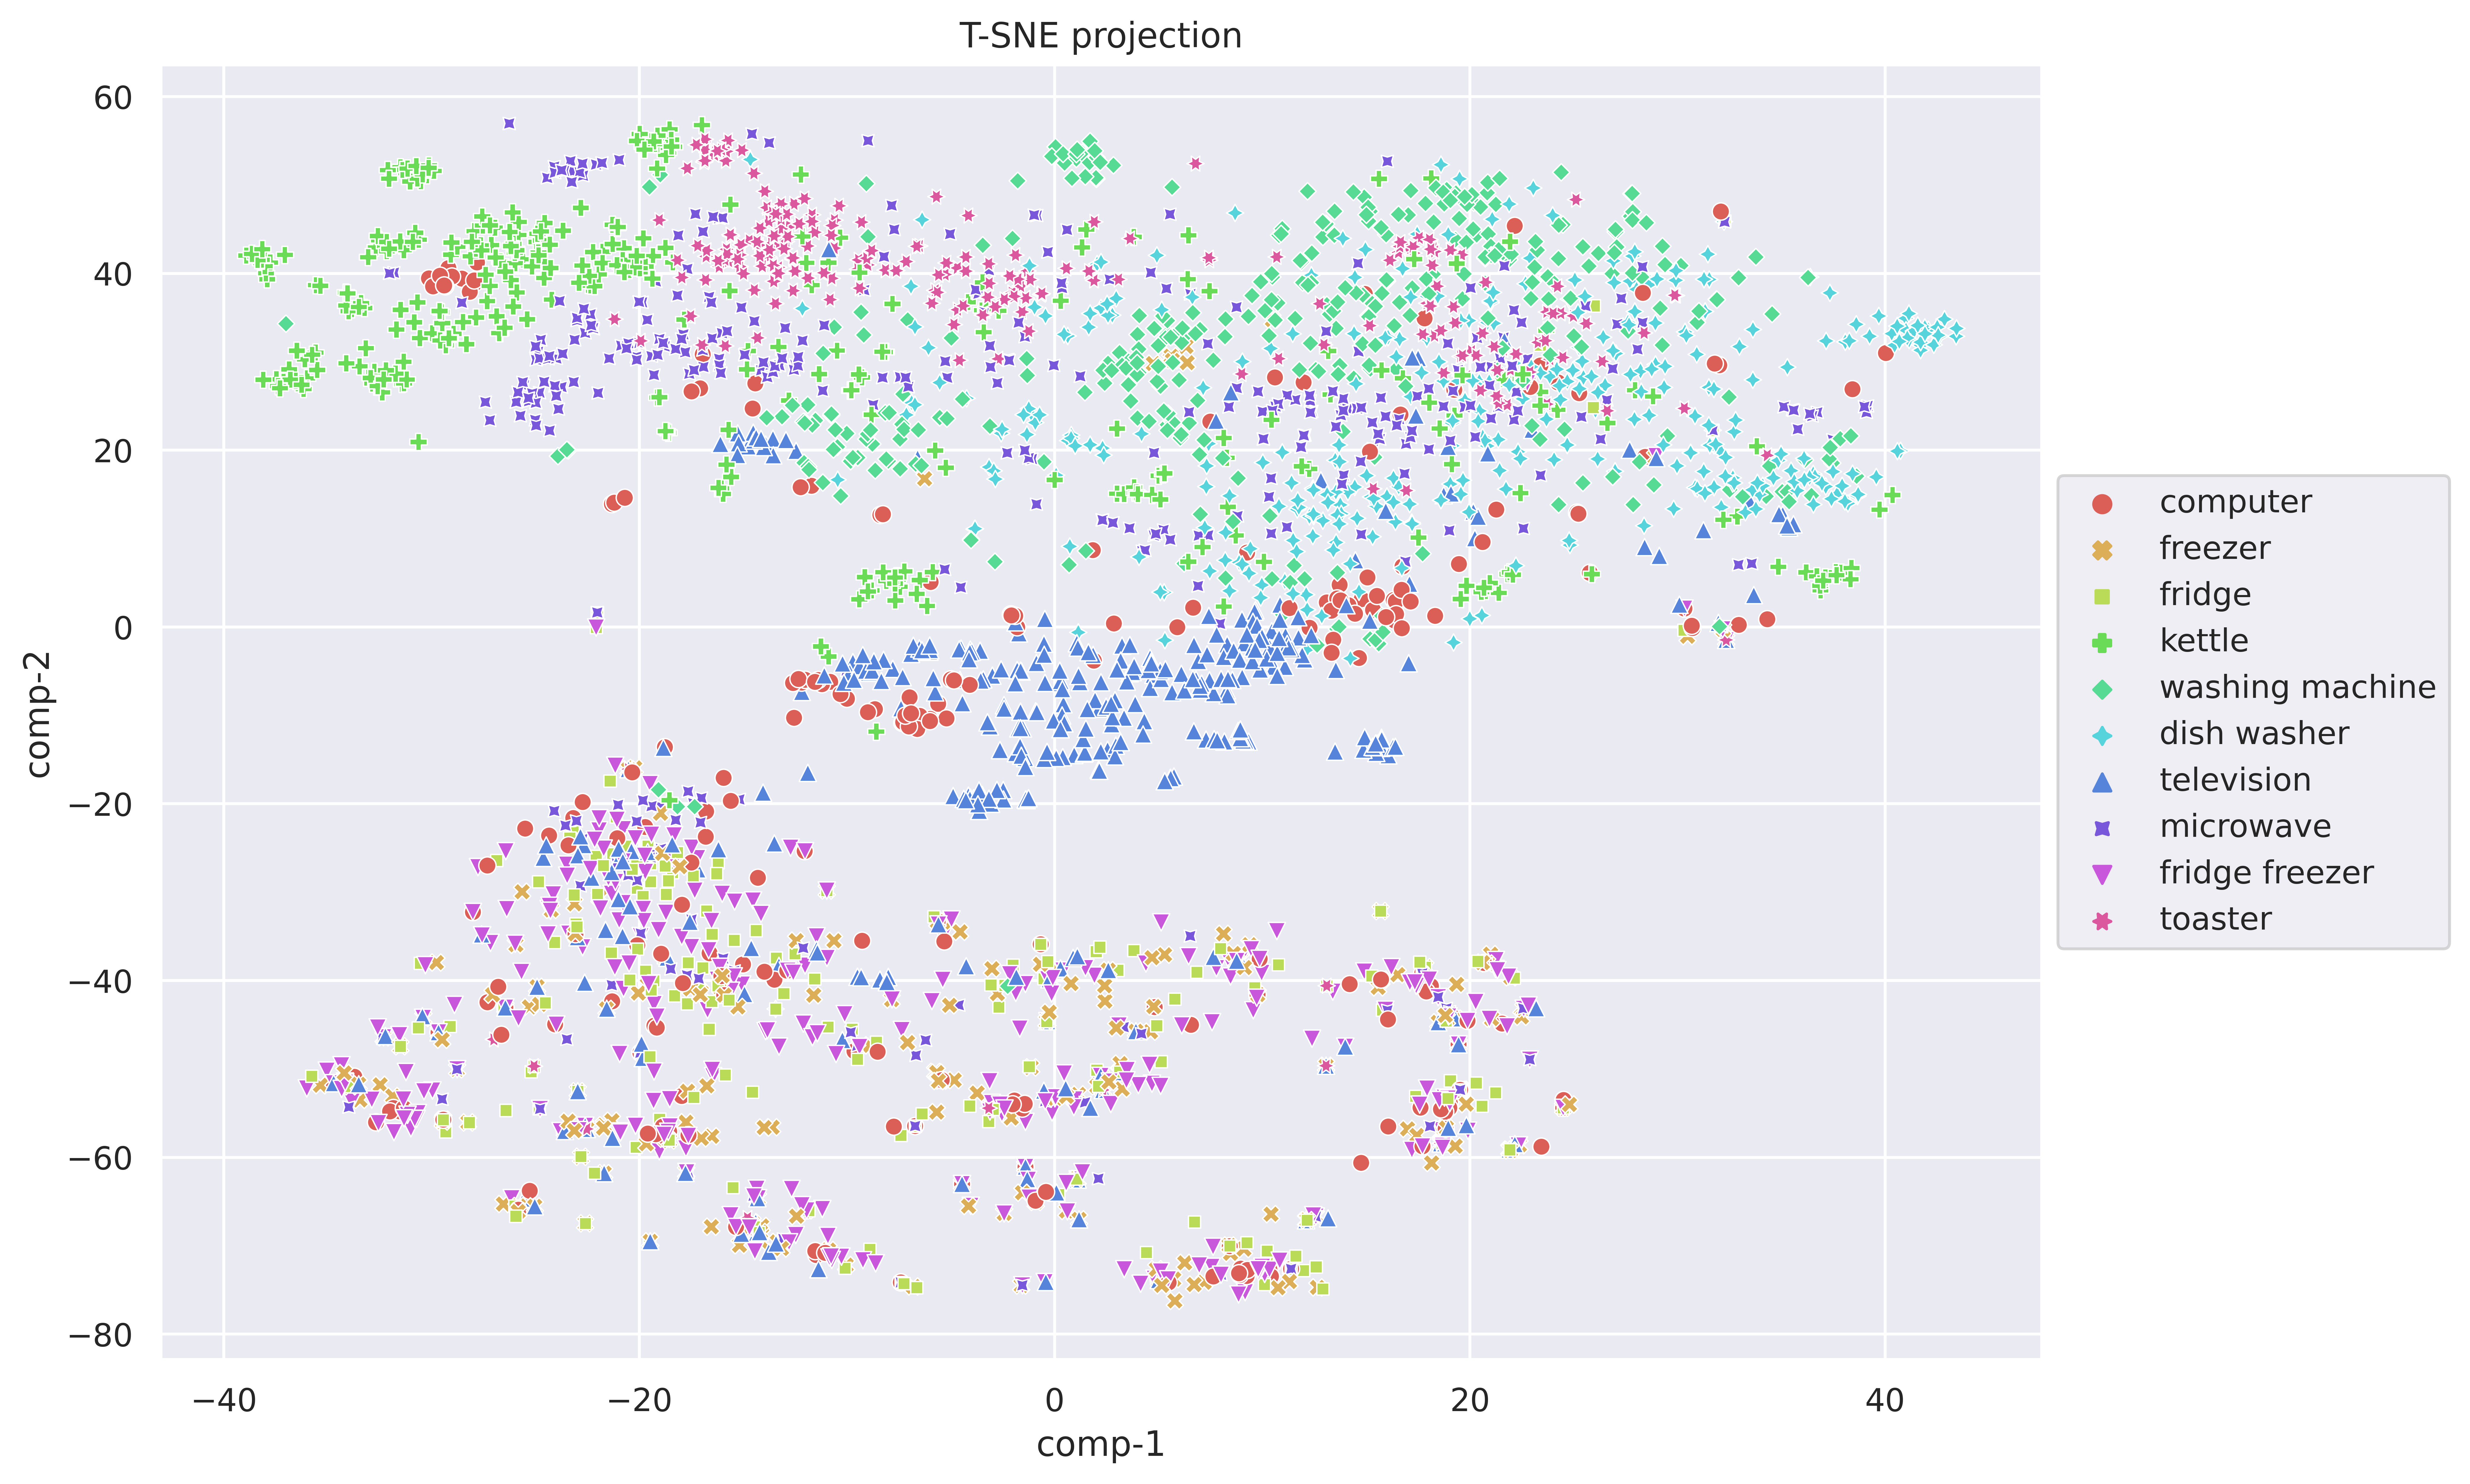
\includegraphics[width=1.2\textwidth]{Figures/TSNE/TSNE_results/all/scatter_all_all_reduced_max.png}
	\label{fig:tsne_papb_scatter_all_reduced}
\end{figure}

\begin{figure}[H]
	\centering
	\caption{"Per appliance data for refit buildings images"}
	\includegraphics[width=.9\textwidth]{Figures/TSNE/TSNE_results/all/img_scatter_allall_reduced_max.png}
	\label{fig:tsne_papb_img_scatter_all_reduced}
\end{figure}

\subsection{group appliances}

\begin{figure}[H]
	\centering
	\caption{"Per appliance per building data for all buildings"}
	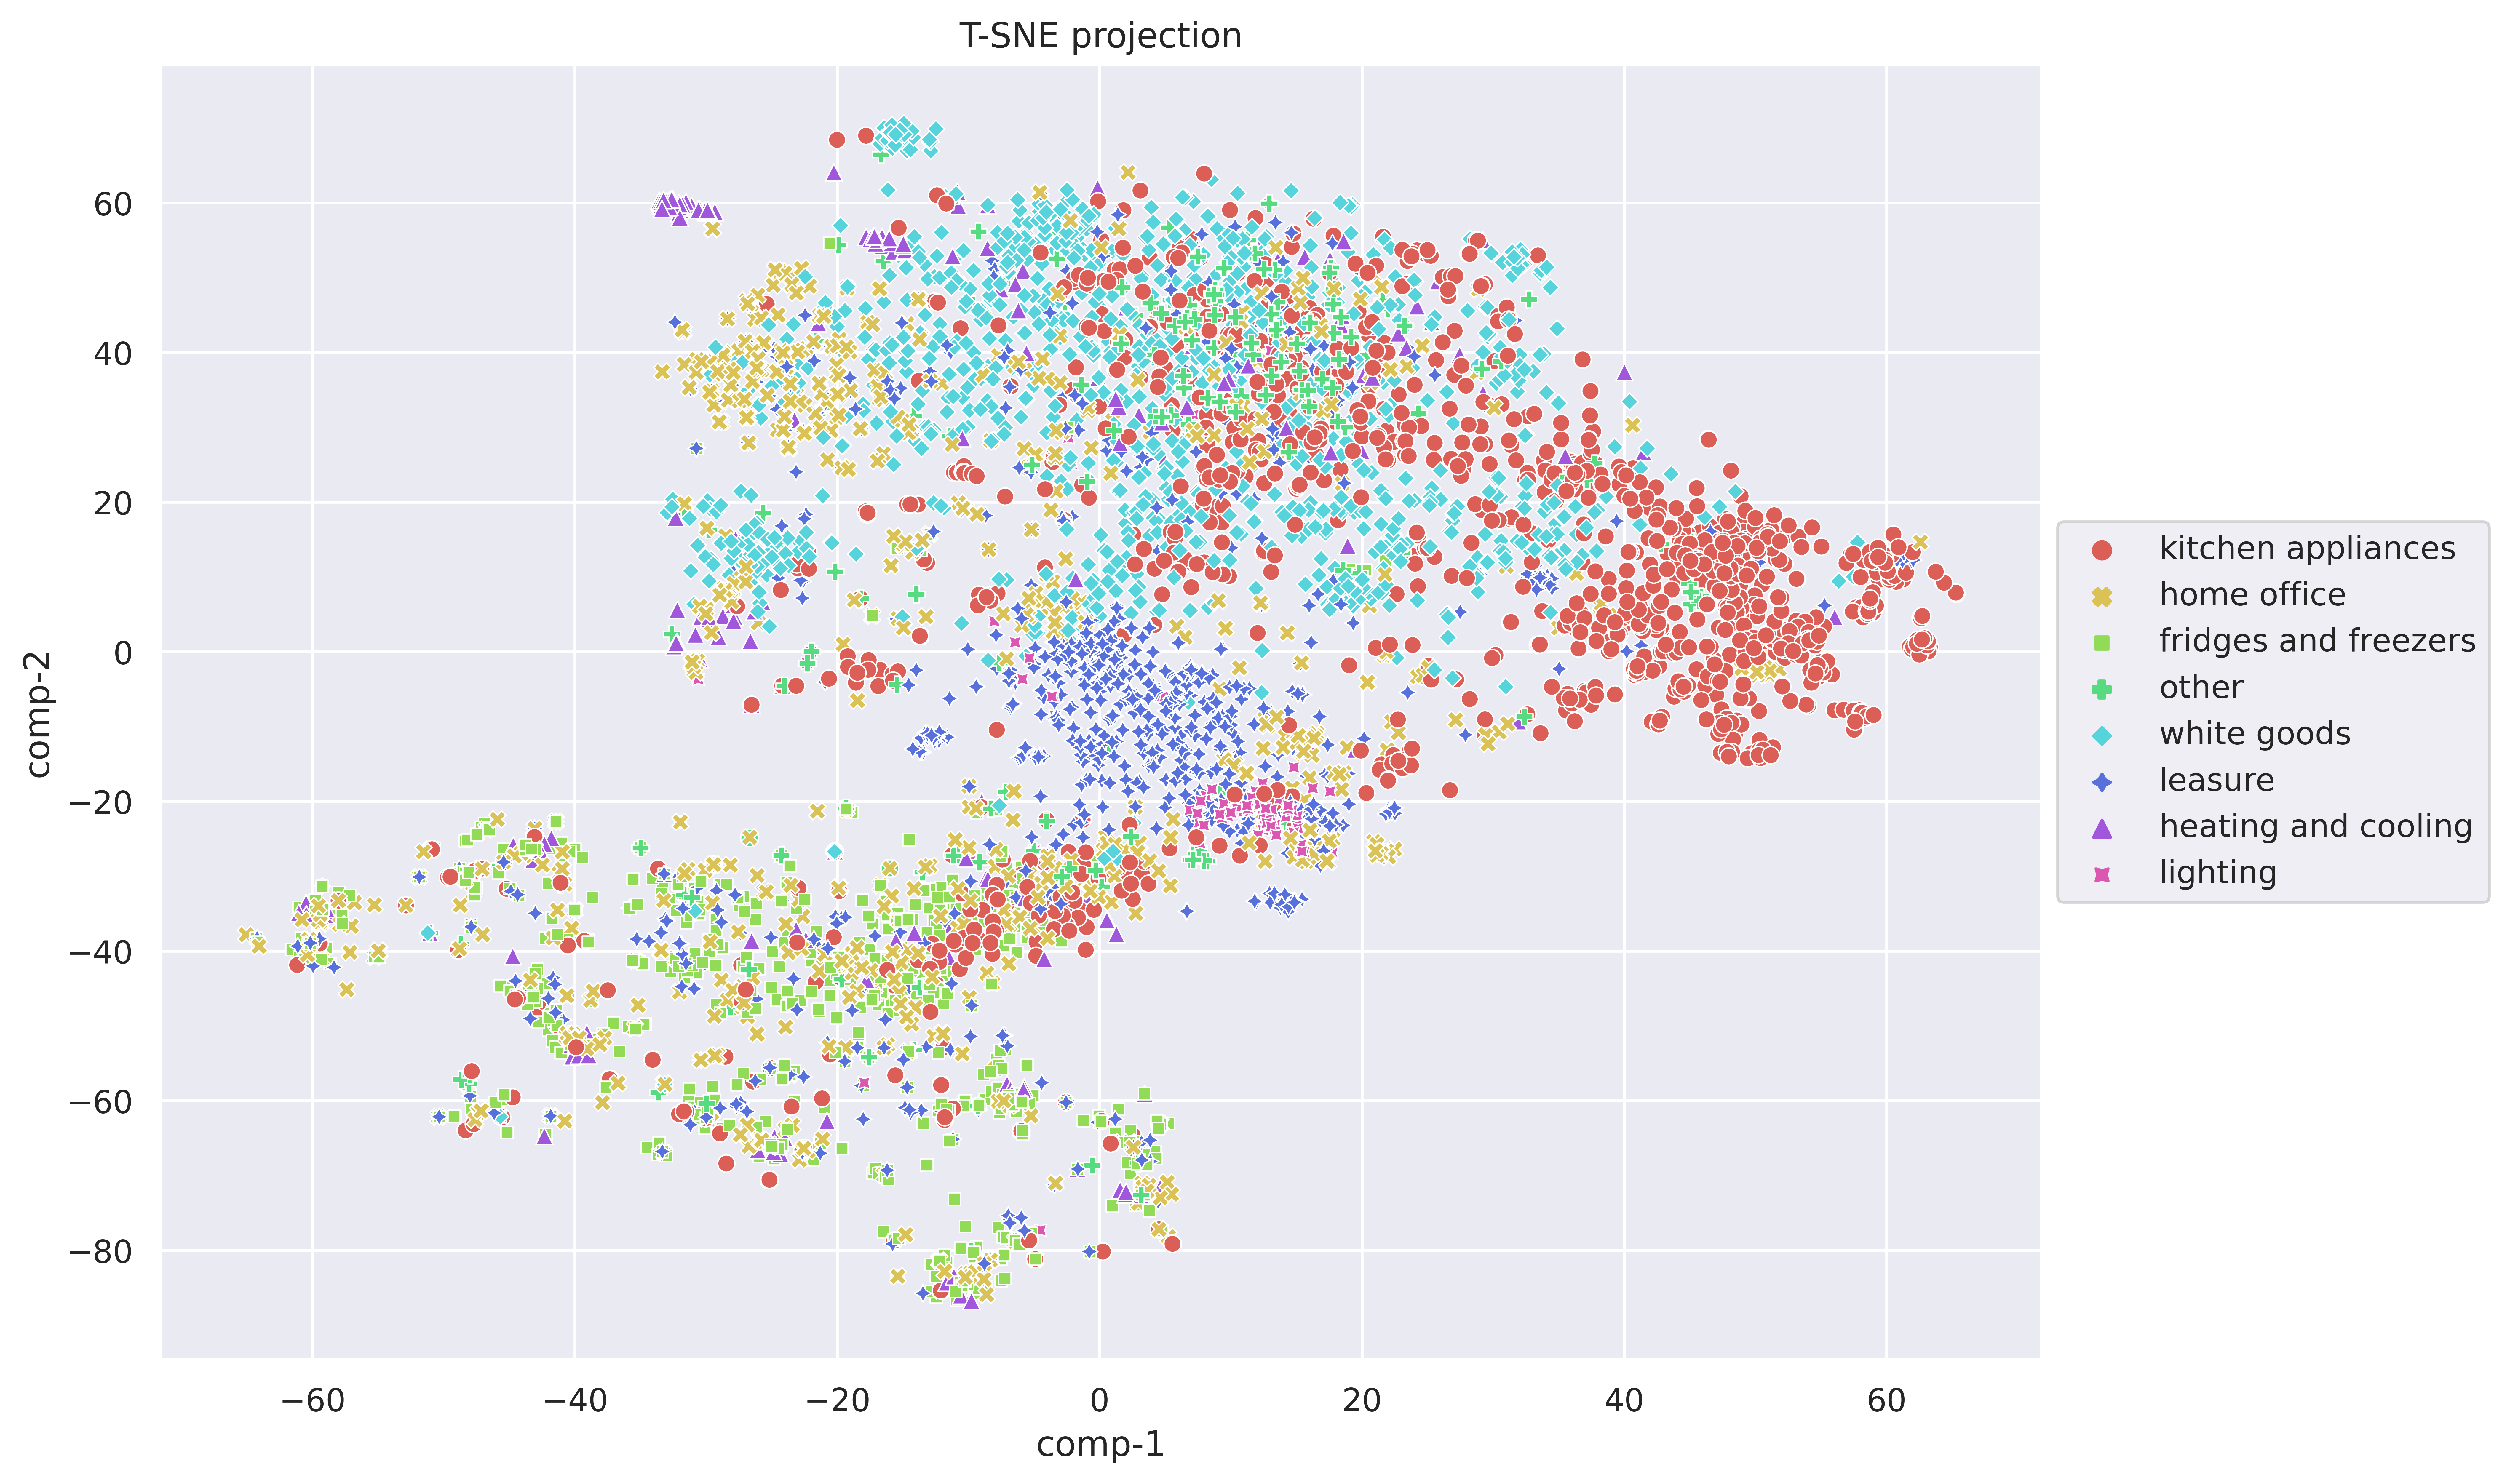
\includegraphics[width=1.2\textwidth]{Figures/TSNE/TSNE_results/all/scatter_all_all_groups.png}
	\label{fig:tsne_papb_scatter_all_groups}
\end{figure}

\begin{figure}[H]
	\centering
	\caption{"Per appliance data for refit buildings images"}
	\includegraphics[width=.9\textwidth]{Figures/TSNE/TSNE_results/all/img_scatter_all_all_groups.png}
	\label{fig:tsne_papb_img_scatter_all_groups}
\end{figure}


\subsection{filter low entropy}

\begin{figure}[H]
	\centering
	\caption{"Per appliance per building data for all buildings"}
	\includegraphics[width=1.2\textwidth]{Figures/TSNE/TSNE_results_entropy/all/scatter_all_all.png}
	\label{fig:tsne_papb_scatter_ent_all_groups}
\end{figure}

\begin{figure}[H]
	\centering
	\caption{"Per appliance per building data for all buildings"}
	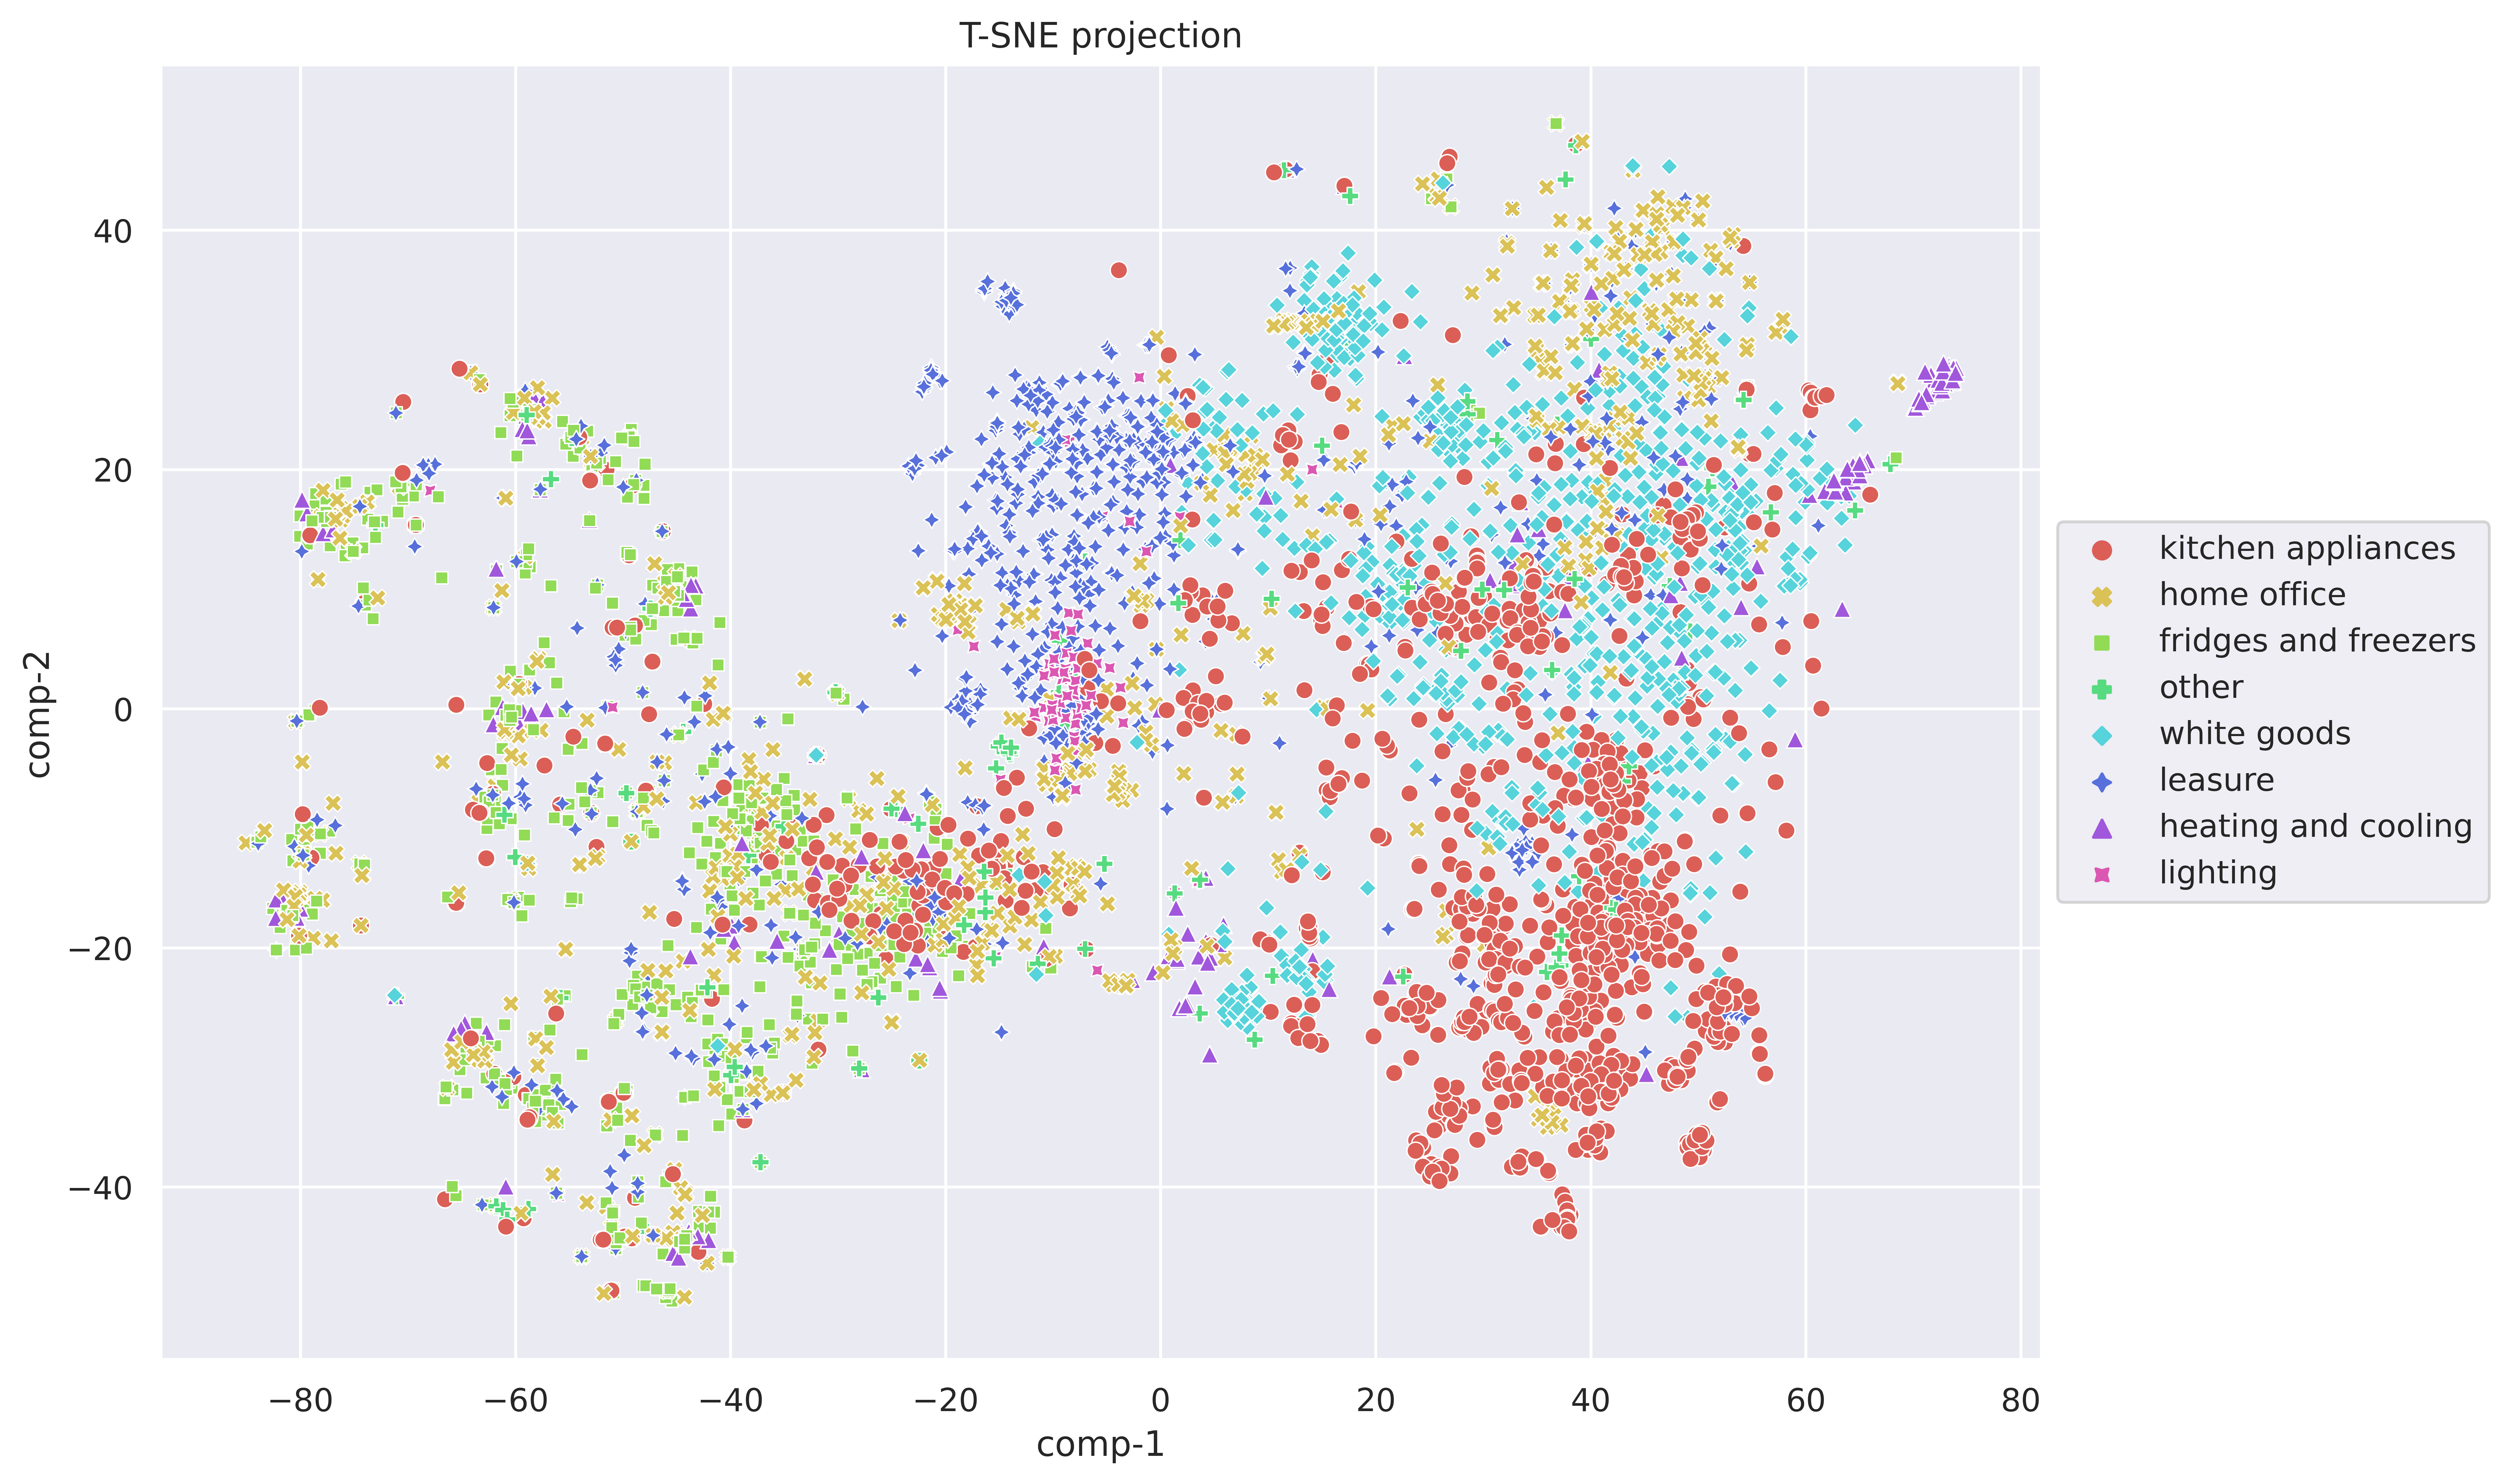
\includegraphics[width=1.2\textwidth]{Figures/TSNE/TSNE_results_entropy/all/scatter_all_all_groups.png}
	\label{fig:tsne_papb_img_scatter_ent_all_groups}
\end{figure}


\subsection{single buildings}

\begin{figure}[H]
	\centering
	\caption{"Per appliance per building data for all buildings"}
	\includegraphics[width=1.2\textwidth]{Figures/TSNE/TSNE_results/refit/scatter_refit_8.png}
	\label{fig:tsne_papb_scatter_ent_refit8}
\end{figure}

\begin{figure}[H]
	\centering
	\caption{"Per appliance data for refit buildings images"}
	\includegraphics[width=.9\textwidth]{Figures/TSNE/TSNE_results/refit/img_scatter_refit8.png}
	\label{fig:tsne_papb_img_scatter_ent_refit8}
\end{figure}


\subsection{per appliance per building}
\subsubsection{Bag off appliances}

\begin{figure}[H]
	\centering
	\caption{"Per appliance per building data for all buildings"}
	\includegraphics[width=.8\textwidth]{Figures/TSNE/TSNE_BOA/refit/scatter_refit_all.png}
	\label{fig:tsne_boa_scatter_refit8}
\end{figure}

\begin{figure}[H]
	\centering
	\caption{"Per appliance data for refit buildings images"}
	\includegraphics[width=.9\textwidth]{Figures/TSNE/TSNE_BOA/refit/img_scatter_refitall.png}
	\label{fig:tsne_boa_img_scatter_refit8}
\end{figure}